\begin{center}
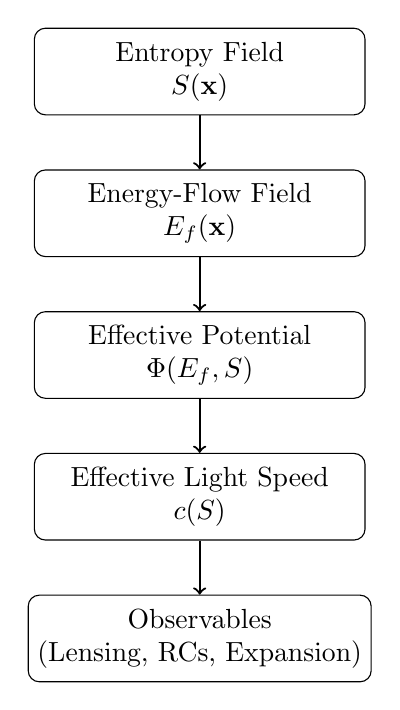
\begin{tikzpicture}[
    node distance=1.8cm,
    box/.style={
        rectangle,
        draw=black,
        rounded corners,
        minimum width=4.2cm,
        minimum height=1.1cm,
        align=center
    },
    arrow/.style={->, thick}
]

% Nodes
\node[box] (S)         {Entropy Field \\ $S(\mathbf{x})$};
\node[box, below of=S] (Ef)        {Energy-Flow Field \\ $E_f(\mathbf{x})$};
\node[box, below of=Ef] (Phi)     {Effective Potential \\ $\Phi(E_f,S)$};
\node[box, below of=Phi] (cS)     {Effective Light Speed \\ $c(S)$};
\node[box, below of=cS] (Obs)     {Observables \\ (Lensing, RCs, Expansion)};

% Arrows
\draw[arrow] (S)   -- (Ef);
\draw[arrow] (Ef)  -- (Phi);
\draw[arrow] (Phi) -- (cS);
\draw[arrow] (cS)  -- (Obs);

\end{tikzpicture}
\end{center}
